\section{Confidence-guided System Design}

This section delves into the technical aspects of confidence guidance within Auto311. Firstly, we explain the method to derive confidence scores from the machine learning models. Secondly, we elucidate the purpose of the generated confidence scores within the workflow.

% In this section, we discuss the technical details of the confidence guidance in Auto311. First, we explain the applied method to obtain the confidence score behind the machine learning models. Second, we illustrate the role of the generated confidence scores in the workflow.

\begin{figure*}[t]
    \centering
    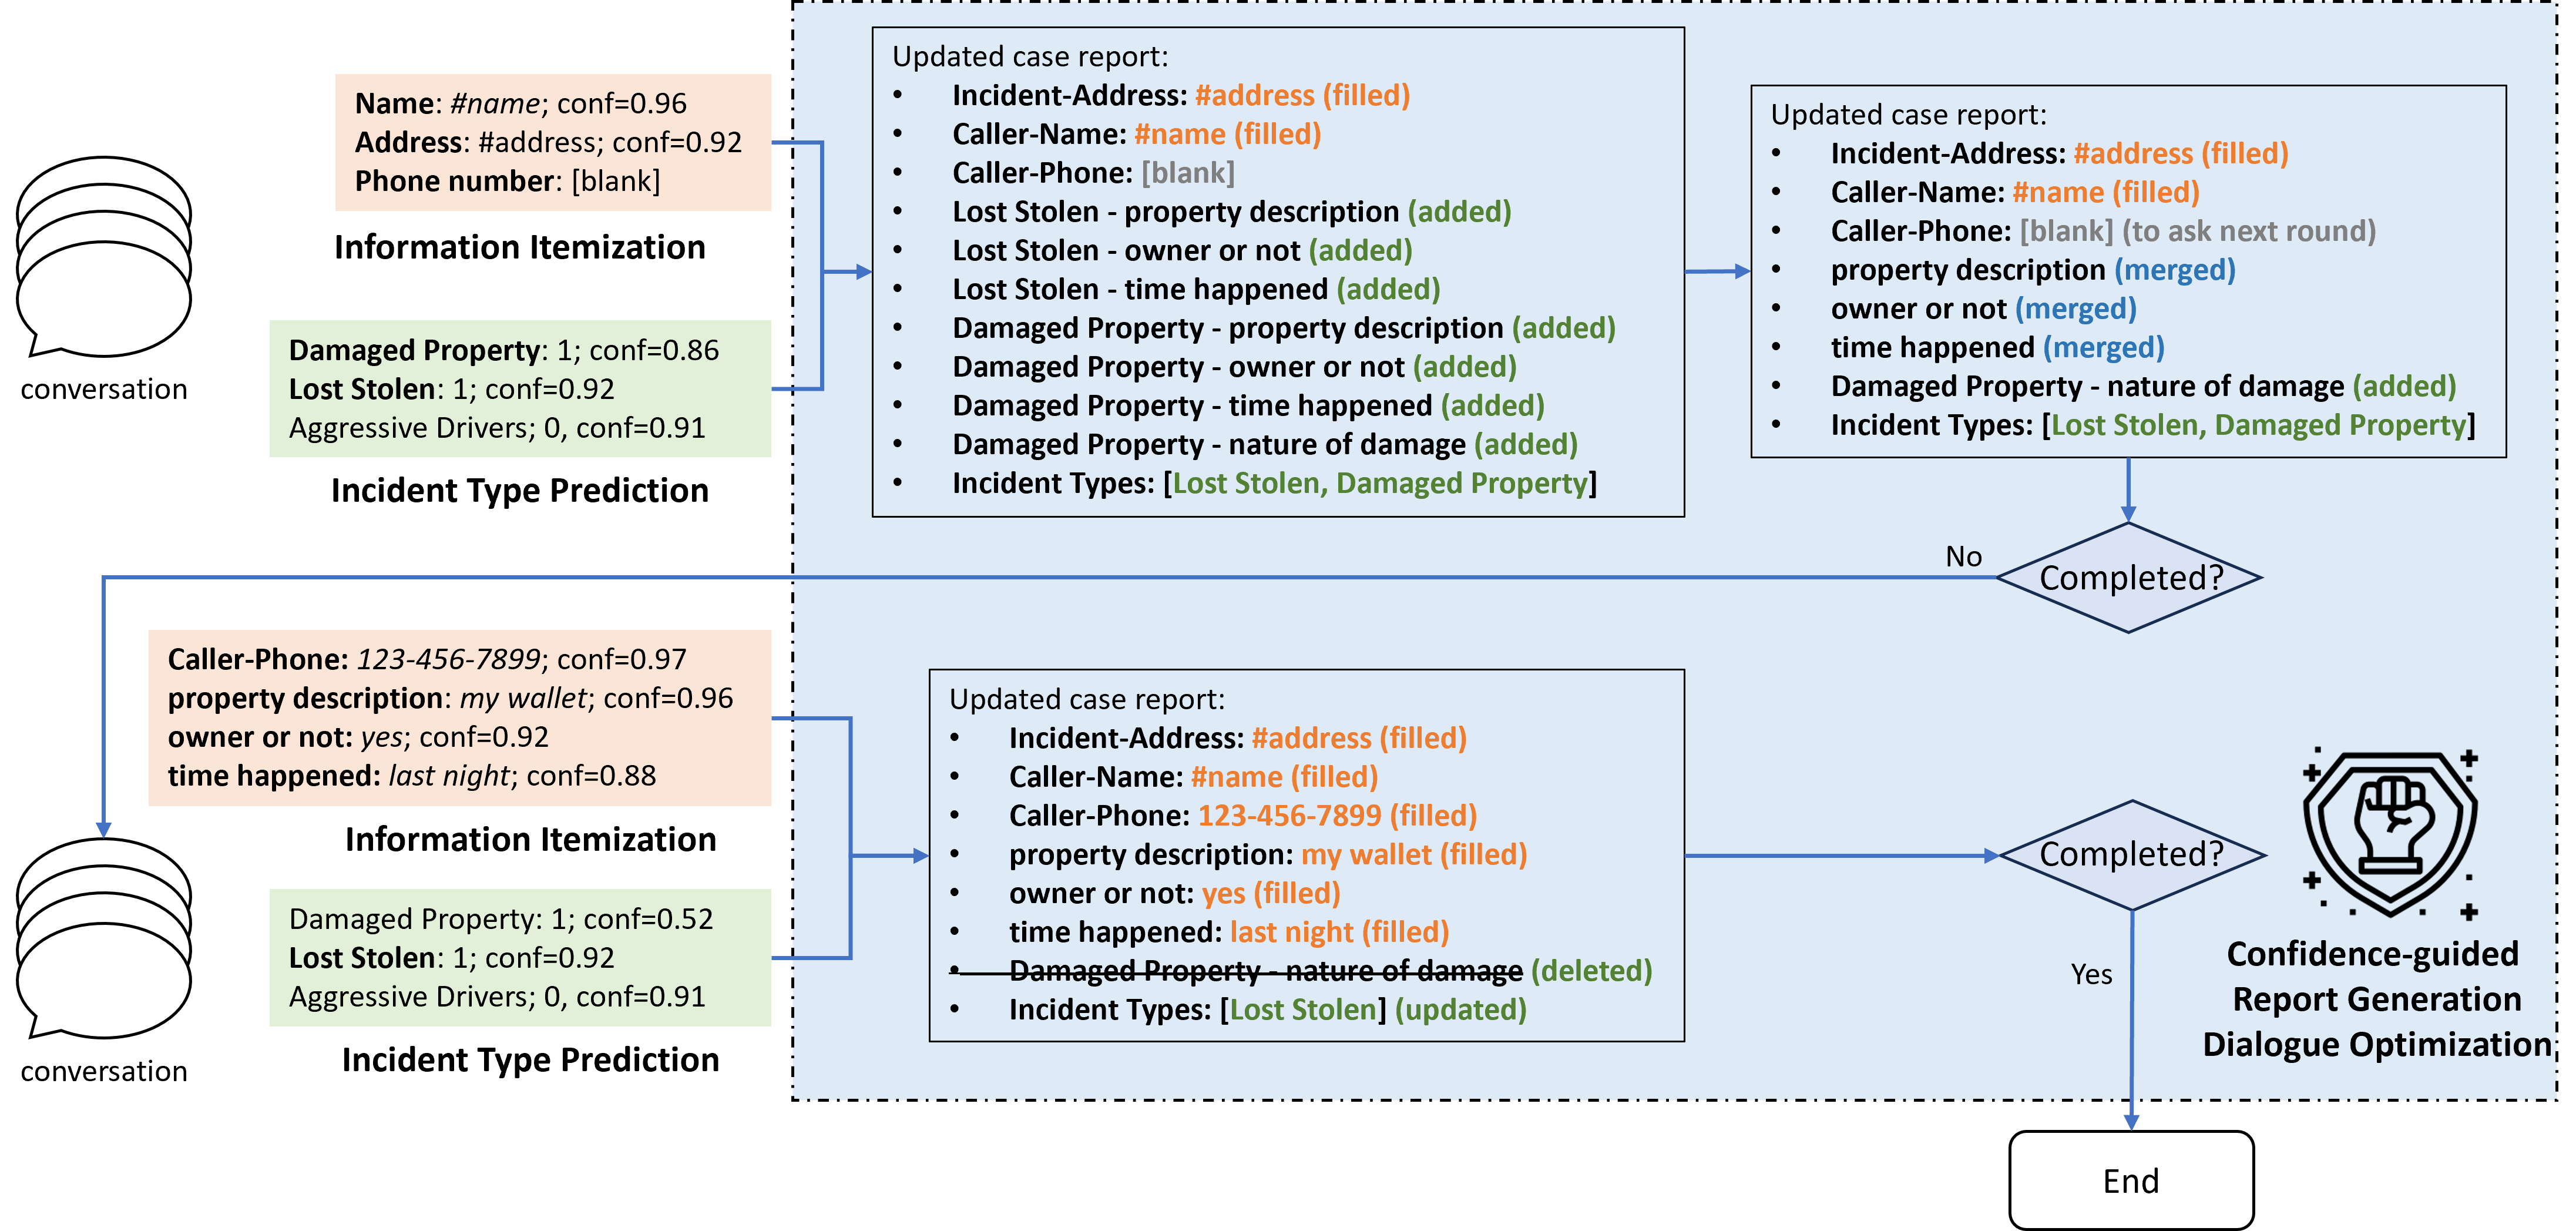
\includegraphics[width=0.9\textwidth]{figures/case_study.png}
    \caption{A General Case Study in Confidence Guidance}
    \label{fig:case_study}
    \vspace{-0.5cm}
\end{figure*}

\subsection{Confidence Measurement}

We define confidence as consistency over multiple trials with the same inputs. We leverage Monte Carlo Dropout\cite{gal2016dropout, ma2021predictive} to generate the confidence prediction. Specifically, dropout was set as active at test time and assesses consistency across trials to obtain scores. Preset thresholds determine if outputs are confident - meeting or exceeding the threshold means confident. Auto311 applies machine learning models to handle two major tasks component-wisely: incident type prediction and information itemization. Here we detail Auto311's approach to measuring confidence.

% Following the definition of confidence score in machine learning as ``the internal consistency with same input after multiple trials'', we apply a similar structure in \cite{ma2021predictive} -- leaving the dropout layer active during testing and calculating the consistency over multiple trials to obtain a confidence score. We set up confidence thresholds -- if the confidence score remains at the threshold or higher, the output is deemed confident. Auto311 applies machine learning models to handle two major tasks component-wisely: incident type prediction and information itemization. Here we detail Auto311's approach to measuring confidence.

\subsubsection{Confidence in Incident Type Prediction}

To address potential multiple incident types within a call, we employ a multi-layer hierarchy structure coupled with a bootstrap-like process. The initial layer of this structure involves training a neural network to assess if the present context corresponds to the most common incident type. Subsequently, the second layer trains another neural network to determine if the context aligns with the second most frequent incident type, excluding the previously identified type. This pattern continues for subsequent types. As a result, (1) the structure can identify all possible incident types within a call; (2) each category operates independently, facilitating future adjustments based on new data or expansion to more categories. At runtime, we establish confidence scores by measuring consistency across output distributions for the same input, utilizing active dropout to quantify prediction uncertainty. The hierarchical cascade structure adeptly handles multiple types, while confidence scoring measures prediction certainty.

% To handle the potential multiple incident types in each call, we apply a multi-layer hierarchy structure with a bootstrap-like procedure. The first layer of the multi-layer classification structure contains a neural network trained to determine if the current context belongs to the most prevalent incident type. Subsequently, the second layer involves training a separate neural network to ascertain if the current context corresponds to the incident type with the second highest frequency after excluding the previous type from the training set, continuing in this manner. Consequently, (1) the overall structure can identify all potential incident types from an ongoing call; (2) each category avoids interfering with others, enabling future fine-tuning on new data samples or expansion with additional categories. We obtain confidence scores at runtime by measuring consistency among output distributions with the same input, keeping dropout active. This quantifies uncertainty in the predictions. The hierarchical cascade structure flexibly handles multiple types, while the confidence scoring quantifies prediction certainty.

\subsubsection{Confidence in Information Itemization}

% Drawing from the machine learning concept of a confidence score, defined as the consistency when testing the same input multiple times, we adopt a similar approach as seen in \cite{ma2021predictive}. This involves keeping the dropout layer active during testing, calculating consistency across multiple trials, and deriving a confidence score. We establish confidence thresholds: if the score equals or surpasses the threshold, the output is considered confident. Auto311 employs machine learning models for two key tasks: predicting incident types and handling information itemization. In this context, we elaborate on how Auto311 gauges the confidence for each task component.

Regarding textual outputs for information itemization, determining confidence necessitates a consistency assessment between texts. Traditional text comparison methods often prioritize aspects like edit distances and length. See details in Related Work. However, our collaboration with DEC underscores the value of succinct outputs with ample details for case reports. Consider the scenario where the module generates ``on the 2525 West End Ave'' while the ground truth is ``2525 West End Ave.'' Traditional methods yield low scores, such as 0.5 from BLEU-bigram. However, when dispatchers gather incident location details, these outputs should exhibit high consistency due to matching location keywords and similar semantics. To address this, we adopt a new approach. For keywords, we employ an unsupervised state-of-the-art keyword extractor \cite{campos2018yake} to extract key segments from model outputs. The overlap between keyword segment lists is calculated. For semantics, we utilize SentenceBERT \cite{reimers-2019-sentence-bert} to project each output into a latent space, assessing the similarity between represented textual string lists. The overall score, calculated via Polyak averaging (p=0.2), integrates keyword overlaps and embedding distances. This metric enables us to gauge consistency and generate a confidence score.

% When it comes to textual outputs in information itemization, it first requires a method to calculate the consistency between texts before a confidence score is finally measured. Traditional text comparison approaches primarily emphasize features including edit distances and length. But throughout the collaboration with the local call center team, we consider concise outputs with ample details more useful for information itemization in the case report. For instance, if the module generates ``on the 2525 West End Ave'' but the ground truth is ``2525 West End Ave'', traditional text comparison methods furnish low scores, e.g. 0.5 from BLEU-bigram. Critically, when dispatchers gather incident location information, these outputs should exhibit high consistency since both contain identical location keywords and similar semantics. Thus, here, for keywords, we leverage an unsupervised state-of-the-art keyword extractor \cite{campos2018yake} to extract key segments from model outputs and calculate the overlap between keyword segment lists. For semantics, we apply SentenceBERT \cite{reimers-2019-sentence-bert} to project each output into a latent space, calculating the similarity between represented textual string lists. The overall score calculates using Polyak averaging, p=0.2, based on keyword overlaps and embedding distances. With the help of the text comparison metric, consistency now can be obtained and a confidence score can be generated under this scenario.

\subsection{Report Generation and Dialogue Optimization}

Auto311 is designed to be confidence-guided. With maximum confidence guaranteed, it (1) dynamically updates case reports at every turn of the conversation and (2) guides the follow-up conversation based on the generated case report. See Figure \ref{fig:sys_logic} for more detailed system logic. 

Confidence drives precise report completion via information itemization. Using the latest caller utterance, it populates report details. Textual output confidence is determined through text comparison. As in Figure \ref{fig:sys_logic}, uncertainty ($conf_1 \leq \lambda_1$) prompts Auto311 to seek clarification for guiding questions, capped at three turns before handover control. Confidence ($conf_1 > \lambda_1$) skips further dialogue optimization for filled fields. Confidence also aids the incident type prediction module's adaptability and report efficiency. Using complete utterance context, it predicts likely incident types. As shown in Figure \ref{fig:sys_logic}, low confidence ($conf_2 \leq \lambda_2$) excludes uncertain predictions from reports. High confidence ($conf_2 > \lambda_2$) incorporates predictions. Systemically, prediction persists each turn, even post early confident identification. This iterative process tracks trends in types and scores, updating reports on confidence drops ($conf_2 \leq \lambda_2$). Confidence-driven adaptation detects and responds to evolving incident types during calls, further updating reports.

% Confidence guides high-quality case report completion through information itemization. Taking the latest caller utterance, it outputs details for relevant report fields. As explained, text comparison determines confidence for textual outputs. As shown in Figure \ref{fig:sys_logic}, if uncertain about itemized info ($conf_1 \leq \lambda_1$), Auto311 prompts clarification if fields guide subsequent questions, capped at 3 turns before handover control is triggered and an operator steps in. When confident ($conf_1 > \lambda_1$), filled fields are excluded from further dialogue optimization. Confidence quantification thus optimizes itemization to complete reports more effectively.

% Confidence is a key factor guiding the accurate completion of case reports through information itemization. The module takes the most recent caller utterance as input and produces itemized information for the relevant fields in the case report as output. As explained earlier, the confidence score for text-based outputs is determined through text comparison. If Auto311 lacks certainty about the itemized information, it prompts the caller for clarification when $conf_1 \leq \lambda_1$, provided the fields guide subsequent questions. Our system limits caller clarification to three turns at most, after which a live operator steps in. Conversely, when $conf_1 > \lambda_1$, Auto311 is confident in the provided itemized information, leading to the fulfillment of the answered fields and exclusion from future dialogue optimization.



% Confidence also enables the incident type prediction module to adapt to evolving categories and generate reports more effectively. Taking the full utterance context, it predicts the most likely types. As illustrated in Figure \ref{fig:sys_logic}, low confidence scores ($conf_2 \leq \lambda_2$) mean uncertainty, so those predictions are excluded from report generation. High confidence ($conf_2 > \lambda_2$) incorporates predicted types into created reports. At a system level, prediction stays engaged every turn, even after confident early identification. This iterative checking empowers Auto311 to monitor trends in types and scores - a drop ($conf_2 \leq \lambda_2$) triggers excluding fields tied to uncertain types, updating the report. Confidence-guided adaptation allows detecting and responding to shifting incident types during the call to further update reports.

% Confidence serves as a guiding principle for the incident type prediction module, allowing it to dynamically adapt to evolving incident categories and generate case reports more effectively. The module takes the overall utterance as input and produces the most likely incident type(s) as output. When Auto311 predicts incident types with a confidence score below the threshold $conf_2 \leq \lambda_2$, it signifies uncertainty in the prediction. Consequently, such predictions are not incorporated into the report-generation process. Conversely, when $conf_2 > \lambda_2$, the predicted incident types are used to generate case reports with specific fields tailored to those types. At a system level, Auto311 maintains the incident type prediction module's engagement in every conversational turn to ensure awareness of the ongoing context. This holds true even when earlier turns have confidently identified an incident type. This approach empowers Auto311 to monitor trends in incident types and their corresponding confidence scores. If the confidence score drops below the threshold ($conf_2 \leq \lambda_2$), indicating decreased certainty in the incident type prediction, Auto311 adjusts the case report by excluding fields highly tied to the specific incident type. This ability allows Auto311 to detect and respond to changes in caller-identified incident types during the conversation, thus updating the case report accordingly.

% Confidence guides the incident type prediction module to dynamically adjust to the shifting incident types and more appropriately generate the case report. The input of the incident type prediction module is the overall caller utterance and the output is the most likely incident type(s). When Auto311 predicts the incident types with a low confidence score $conf_2 \leq \lambda_2$, it implies Auto311 is not fully certain about the prediction. In this case, the prediction is not adopted for report generation. Oppositely, when $conf_2 > \lambda_2$, the predicted incident types are further utilized to generate the case report with type-specific fields. Meanwhile, at a system level, Auto311 keeps the incident type prediction module active at every turn of the conversation to make it aware of the overall context, even when previous turns have confirmed one incident type with a high confidence score. By doing so, Auto311 is capable of tracking the trend of both incident types and the corresponding confidence scores. If the confidence score decreases lower than the threshold, when $conf_2 \leq \lambda_2$, indicating the incident type prediction module is no longer certain about the given type, Auto311 modifies the case report by dropping fields highly specific to the incident type. Thus, when the caller shifts the incident types during the call, Auto311 detects the shift and adjusts the case report using the updated incident type.

Previous component confidence scores further optimize future dialogues. In the case study illustrated in Figure \ref{fig:case_study}, when a new caller utterance is received, Auto311 identifies fields to complete in the case report (e.g., incident-address, caller-name, caller-phone). High-confidence completion marks them as done. Unfinished fields guide subsequent questions (e.g., requesting a callback number if caller-phone is missing). Concurrently, incident type is confirmed if confidence surpasses a set threshold (0.85 in Figure \ref{fig:case_study}). With the type established, specialized fields are identified (e.g., property description for lost/stolen cases), updating the report. Auto311 then prioritizes shared general fields (e.g., property description, time, ownership status), streamlining dialogue to focus initially on universal details. This avoids asking about the damage nature before finalizing the incident type, which applies only to damaged property cases. This optimization confirms type(s) with more context. In the example, the next turn's details indicate a shift to "lost/stolen" only. The report is updated accordingly. The dialogue concludes when all report fields are complete. Confidence scoring thus optimizes the flow by collecting universal details first and adapting to emergent incident types.


% The confidence scores from previous components play a significant role in optimizing future dialogue. As illustrated in the case study \ref{fig:case_study}, when receiving a new caller utterance, Auto311 first identifies fields to fill in the case report (e.g. incident-address, caller-name, caller-phone). High confidence completion of these fields marks them as finished. Remaining incomplete fields guide the next questions (e.g. asking for callback number if caller-phone is missing). Simultaneously, the incident type is confirmed if its confidence exceeds a preset threshold (0.85 in the figure). With the type established, Auto311 identifies specialized fields needed (e.g. property description for lost/stolen cases). The report is updated accordingly. Following this, Auto311 consolidates and prioritizes more general fields shared across incident types (e.g. property description, time, ownership status). This streamlines the dialogue to focus initially on universal information before specific inquiries. For instance, the system avoids asking about the nature of damage before finalizing the incident type, since it is identical to only damaged property cases. This optimization provides additional context to confirm type(s). In the example, in the next turn, the caller supplies missing details that indicate shifting to ``lost/stolen'' only. The report is updated based on the revised predictions. The dialogue concludes when all report fields are complete. In summary, confidence scoring enables optimizing the flow to gather universal details first, then adapt based on emergent incident types.

% The confidence scores produced by the previous components play a significant role in optimizing future dialogue, as illustrated in a general case study in Figure \ref{fig:case_study}. Upon receiving a new caller utterance, Auto311 initially identifies the fields that need to be filled in the case report. For example, in Figure \ref{fig:case_study}, these could include incident-address, caller-name, and caller-phone. If these pieces of information are collected with high confidence, the corresponding fields are marked as completed. The fields that remain incomplete guide the ongoing conversation, determining the next questions to be posed. For instance, if caller-phone is missing (as indicated by the gray marking in the figure), the next question might be, ``What is your preferred callback number?'' Simultaneously, the incident type is confirmed if its confidence score surpasses the preset threshold, represented as 0.85 in Figure \ref{fig:case_study}. Once the incident type is established, Auto311 refers to the call center's protocol to identify fields requiring type-specific details. In the figure, the prevalent incident types are ``damaged property'' and ``lost/stolen property.'' Accordingly, the case report is augmented with specialized fields such as ``lost stolen - property description'' and ``damaged property - nature of damage.'' Following this update, Auto311 proceeds to consolidate and prioritize less specific fields. For instance, both ``damaged property'' and ``lost stolen property'' incidents necessitate common information like property description, time of occurrence, and ownership status. Hence, Auto311 combines and gives priority to these shared fields. The outcome is a more streamlined dialogue that initially focuses on gathering universal information, postponing highly specific inquiries until incident types are definitively determined. For example, as shown in the second turn of Figure \ref{fig:case_study}, the system avoids inquiring about the nature of damage before the incident type is finalized. This optimized dialogue approach also affords Auto311 additional context to confirm the incident type(s). In the subsequent turn of conversation depicted in Figure \ref{fig:case_study}, the caller not only supplies the missing phone number but also provides details about the related property and the time of the incident. This new information indicates a shift in incident type to ``lost stolen'' only. Consequently, the case report is updated based on the revised module outputs. The dialogue concludes when all fields in the case report are filled.

% The confidence emitted by the components is also utilized for future dialogue optimization, see a general case study in Figure \ref{fig:case_study}. Once a new caller utterance is given, Auto311 first tracks the fields to complete in the case report, e.g., incident-address, caller-name, and caller-phone in Figure \ref{fig:case_study}.  If that information is collected with high confidence, the corresponding fields are marked as completed. The uncompleted fields guide the dialogue by defining the next questions to ask in future turns, e.g., caller-phone is missing, marked grey, and the next question to ask is ``What is your best number for a callback?''. At the same time, the incident type is confirmed if the confidence score exceeds the threshold, set to 0.85 in Figure \ref{fig:case_study}. Once the incident type is confirmed, Auto311 refers to the call center's protocol for fields with type-specific information. As shown in the figure, the most incident types are damaged property and lost/stolen property. Thus, the case report is updated with additional specific fields like the ``lost stolen - property description'' and ``damaged property - nature of damage''. After updating the case report, Auto311 updates the case report by merging and prioritizing less specific fields. For example, in Figure \ref{fig:case_study}, both damaged property and lost stolen property request common information like property description, time happened, and owner or not. Thus, Auto311 merges and prioritizes those common fields. As a result, the future dialogue is optimized and guided to only ask the caller for common fields first without asking highly type-specific questions before the incident types are finalized, e.g., asking ``What is the nature of damage?'' in the second turn in Figure \ref{fig:case_study}. This optimized dialogue also gives Auto311 extra contexts to finalize the incident type(s). For example, in the next turn of conversation in Figure \ref{fig:case_study}, the caller not only provides the missing phone number but also describes the related property and the time when the incident happened. This new utterance implies the incident type is shifted to lost stolen only. The case report is then updated based on the new module outputs. And the dialogue is terminated if all the fields on the case report are completed.

% Once the incident type is confirmed, this module directly refers to the call center's protocol for more specific information that needs to be collected. E.g., if the incident type is confirmed as ``illegal parking'', based on the protocol, more specific information like vehicle description will be needed. After having the necessary information,  Auto311 appends the fields that query the information to the case report, e.g., ``Illegal Parking - Vehicle Description''. When there are multiple incident types confirmed, Auto311 takes care of the fields for multiple incident types. E.g., when the call involves ``damaged property'' and ``lost stolen property'', Auto311 needs to obtain all necessary information for both types, including ``Damage Property - property description'', ``Damaged Property - owner or not'', ``Damaged Property - time happened'', ``Damaged Property - nature of damage'', ``Lost Stolen - property description'', ``Lost Stolen - owner or not'', and ``Lost Stolen - time happened''.  As we can tell, although ``damaged property'' and ``lost stolen property'' are two different incident types, they still share several fields requesting similar information. We define those fields requesting highly overlapped information to be less specific than others. Thus, in our design, Auto311 not only retrieves the specific fields but also rearranges the fields based on how specific they are to the incident types. From the previous example, the first few fields will query the information regarding ``property description'', ``owner or not'', and ``time happened''. By doing so, Auto311 gives the incident type prediction module more context to finalize the incident type. And progressively, see Figure \ref{fig:case_study} for more details, as Auto311 gets more and more certain about the incident type, more and more specific questions regarding the confirmed incident type will be proposed to the caller.


% To handle the potential multiple incident types in each call, we apply a multi-layer hierarchy structure with a bootstrap-like procedure. The first layer of the multi-layer classification structure encompasses training a neural network to determine if the current context belongs to the most prevalent incident type. Subsequently, the second layer involves training a separate neural network to ascertain if the current context corresponds to the incident type with the second highest frequency after excluding the previous type from the training set, continuing in this manner. This structure furnishes each incident type with an individual cascade model. Consequently, (1) the overall structure can identify all potential incident types from an ongoing call; (2) each category avoids interfering with others, facilitating future fine-tuning on new data samples or structure expansion with additional categories.

% % \subsection{Measuring Confidence Scores in Textual Outputs}
% % Following the definition of confidence score in machine learning as ``the internal consistency with same input after multiple trials'', to furnish a confidence score, we apply a similar structure in \cite{ma2021predictive} -- leaving the dropout layer active during testing and calculating the consistency over multiple trials. We also set up confidence thresholds. If the confidence score remains at the threshold or higher, the output is deemed confident.

% % However, when it comes to textual outputs, it first requires a method to calculate the consistency between texts before a confidence score is finally measured. Traditional text comparison approaches predominantly emphasize features including edit distances and length. But throughout the collaboration with the local call center team, we find these features are not completely suitable for this specific non-emergency call-handling task. They consider concise outputs with ample details more useful for information itemization in the case report. For instance, if the module generates ``on the 2525 West End Ave'' but the ground truth is ``2525 West End Ave'', traditional text comparison methods furnish low scores, e.g. 0.5 from BLEU-bigram. Critically, when dispatchers gather incident location information, these outputs should exhibit high consistency since both contain identical location keywords and similar semantics. Thus, here, for keywords, we leverage an unsupervised state-of-the-art keyword extractor \cite{campos2018yake} to extract key segments from model outputs and calculate the overlap between keyword segment lists. For semantics, we apply SentenceBERT \cite{reimers-2019-sentence-bert} to project each output into a latent space, calculating the similarity between represented textual string lists. The overall score calculates using Polyak averaging based on keyword overlaps and embedding distances. With the help of the text comparison metric, consistency now can be obtained and a confidence score can be generated under this scenario.


% % % However, in the information itemization module, it requires a different method to obtain the confidence score. Because the output of the module is no longer a distribution, the outputs come in textual format instead. Thus, measuring consistency between two textual strings becomes necessary. Current text comparison techniques predominantly emphasize features including edit distances and length. However, based on DEC requirements, our module outputs need concision while incorporating ample detail. For instance, if the model generates ``on the 2525 West End Ave'' and ``2525 West End Ave'' from two trials with the same expression, traditional text comparison methods furnish low scores, e.g. 0.5 from BLEU-bigram. Critically, when dispatchers gather incident location information, these outputs should exhibit high consistency since both contain identical location keywords and similar semantics. Hence, a more appropriate method for comparing textual strings is necessary here. Considering the specific demands of this task, we design a consistency metric consisting of two separate keyword and semantic measurements. For keywords, we leverage an unsupervised state-of-the-art keyword extractor \cite{campos2018yake} to extract key segments from model outputs and calculate the overlap between keyword segment lists. For semantics, we apply SentenceBERT \cite{reimers-2019-sentence-bert} to project each output into a latent space, calculating the similarity between represented textual string lists. The overall score calculates using Polyak averaging based on keyword overlaps and embedding distances. With the help of the text comparison metric, consistency now can be obtained and a confidence score can be generated under this scenario.

% \subsection{Confidence-guided System Design}

% Auto311 is designed to be confidence-guided. It is able to, with maximum confidence guaranteed, (1) dynamically generate and complete case reports at every turn of the conversation and (2) guide the follow-up conversation based on the generated case report. See Figure \ref{fig:sys_logic} for more detailed system logic.

% \subsubsection{Iterative Incident Type Checking}

% Auto311 keeps the incident type prediction module active at every turn of the conversation, even when previous turns have confirmed one incident type. By doing so, Auto311 is capable of tracking the trend of both incident types and the corresponding confidence scores. If the confidence score decreases lower than the threshold, indicating the incident type prediction module is no longer certain about the given type, Auto311 modifies the case report by dropping fields highly specific to the incident type. Thus, when the caller shifts the incident types during the call, Auto311 detects the shift and adjusts the case report using the updated incident type.

% \subsubsection{Field Selection and Dialogue Organization}
% Once the incident type is confirmed, this module directly refers to the call center's protocol for more specific information that needs to be collected. E.g., if the incident type is confirmed as ``illegal parking'', based on the protocol, more specific information like vehicle description will be needed. After having the necessary information,  Auto311 appends the fields that query the information to the case report, e.g., ``Illegal Parking - Vehicle Description''. When there are multiple incident types confirmed, Auto311 takes care of the fields for multiple incident types. E.g., when the call involves ``damaged property'' and ``lost stolen property'', Auto311 needs to obtain all necessary information for both types, including ``Damage Property - property description'', ``Damaged Property - owner or not'', ``Damaged Property - time happened'', ``Damaged Property - nature of damage'', ``Lost Stolen - property description'', ``Lost Stolen - owner or not'', and ``Lost Stolen - time happened''.  As we can tell, although ``damaged property'' and ``lost stolen property'' are two different incident types, they still share several fields requesting similar information. We define those fields requesting highly overlapped information to be less specific than others. Thus, in our design, Auto311 not only retrieves the specific fields but also rearranges the fields based on how specific they are to the incident types. From the previous example, the first few fields will query the information regarding ``property description'', ``owner or not'', and ``time happened''. By doing so, Auto311 gives the incident type prediction module more context to finalize the incident type. And progressively, see Figure \ref{fig:case_study} for more details, as Auto311 gets more and more certain about the incident type, more and more specific questions regarding the confirmed incident type will be proposed to the caller.


% Mutual information --> specific level

% After obtaining both finalized outputs and corresponding confidence scores from previous modules, our system takes actions based on those scores, see Figure \ref{fig:sys_logic}. Once the incident type is confirmed, this module directly refers to the call center's protocol for more specific information that needs to be collected. E.g., if the incident type is confirmed as ``illegal parking'', based on the protocol, more specific vehicle-related information will be the brand, color, and license plate number. As a result, more blank fields requesting those information are appended to the case report. The updated case report guides the information itemization module. The system only accepts field-information pairs that obtain confidence scores exceeding the threshold. In other words, with guidance from the confidence score and the finalized incident type, now the system is capable of extending the case report. Meanwhile, by combining the information itemization module with confidence guidance, our system is now able to fulfill the case report by offering field-information pairs with high confidence, see a general case study in Figure \ref{fig:case_study}. We also conclude the following three special cases to fully demonstrate the logic.

% \subsection{Incident Type Prediction}
% \label{subsec:prediction}

% The first layer of the multi-layer classification structure encompasses training a neural network to determine if the current context belongs to the most prevalent incident type. Subsequently, the second layer involves training a separate neural network to ascertain if the current context corresponds to the incident type with the second highest frequency after excluding the previous type from the training set, continuing in this manner. This structure furnishes each incident type with an individual cascade model. Consequently, (1) the overall structure can identify all potential incident types from an ongoing call; (2) each category avoids interfering with others, facilitating future fine-tuning on new data samples or structure expansion with additional categories.

% % To minimize model overhead, freezing of the neural network's main body transpires, with only the downstream fully-connected layers undergoing training for each incident type.

% \subsection{Information Itemization}
% \label{subsec:itemization}

% The information itemization module aims to fill in the blank fields in the case report with critical information from user utterances. Leveraging the ability of existing extractive question-answering frameworks, this module takes the question behind each blank field in the case report as input and outputs the most relevant information by quoting the caller utterance segments. Before training the model, we manually review our dataset and DEC's protocol on different incident types. We annotate the audio transcriptions to form our dataset in field-information pairs, which enables the training of this module. Different from the incident type prediction, which considers all previous contexts, this information itemization module considers only the last caller utterance as context. 

% \subsection{Confidence-guided Report Optimization}
% \label{subsec:confidence}

% This module targets the optimization of the created case report during every turn of the ongoing conversation.

% \subsubsection{Case Report vs Question List}
% It is worth noting that the case report mentioned here is different from the question list in the conversational interface in the following aspects: (1) the question list initially contains 4 questions but the case report initially contains 7 blank fields including the caller's name, the caller's contact number, the location of the incident, the narrative description of the incident, the potential vehicle-related description, the potential property-related description, and the potential suspect-related description; (2) the question list contains questions to ask in the next turns in the conversation, however, the case report consists of blank fields that need to be completed by the information itemization module; (3) the question list can be extended with blank fields with missing or low-confident answers while the case report can be extended by more specific fields under the predicted incident type from the incident type prediction module.

% \subsubsection{Confidence Measurement}

% Following the definition of confidence score in machine learning as ``the internal consistency with same input after multiple trials'', to furnish a confidence score, we apply a similar structure in \cite{ma2021predictive} -- leaving the dropout layer active during testing and calculating the consistency over multiple trials. We also set up confidence thresholds for both incident type prediction and information itemization modules. If the confidence score remains at the threshold or higher, the output is deemed confident.

% In the incident type prediction module, we finalize the result with the prediction with the most appearances within 100 trials. And the confidence score is the percentage of appearances in 100 trials. However, in the information itemization module, it requires a different method to obtain the confidence score. Because the output of the module is no longer a distribution, the outputs come in textual format instead. Thus, measuring consistency between two textual strings becomes necessary. Current text comparison techniques predominantly emphasize features including edit distances and length. However, based on DEC requirements, our module outputs need concision while incorporating ample detail. For instance, if the model generates ``on the 2525 West End Ave'' and ``2525 West End Ave'' from two trials with the same expression, traditional text comparison methods furnish low scores, e.g. 0.5 from BLEU-bigram. Critically, when dispatchers gather incident location information, these outputs should exhibit high consistency since both contain identical location keywords and similar semantics. Hence, a more appropriate method for comparing textual strings is necessary here. Considering the specific demands of this task, we design a consistency metric consisting of two separate keyword and semantic measurements. For keywords, we leverage an unsupervised state-of-the-art keyword extractor \cite{campos2018yake} to extract key segments from model outputs and calculate the overlap between keyword segment lists. For semantics, we apply SentenceBERT \cite{reimers-2019-sentence-bert} to project each output into a latent space, calculating the similarity between represented textual string lists. The overall score calculates using Polyak averaging based on keyword overlaps and embedding distances. With the help of the text comparison metric, consistency now can be obtained and a confidence score can be generated under this scenario.


% \subsubsection{Confidence-guided System Designs}

% After obtaining both finalized outputs and corresponding confidence scores from previous modules, our system takes actions based on those scores, see Figure \ref{fig:sys_logic}. Once the incident type is confirmed, this module directly refers to DEC's protocol for more specific information that needs to be collected. E.g., if the incident type is confirmed as ``illegal parking'', based on DEC's protocol, more specific vehicle-related information will be the brand, color, and license plate number. As a result, more blank fields requesting those information are appended to the case report. The updated case report guides the information itemization module. The system only accepts field-information pairs that obtain confidence scores exceeding the threshold. In other words, with guidance from the confidence score and the finalized incident type, now the system is capable of extending the case report. Meanwhile, by combining the information itemization module with confidence guidance, our system is now able to fulfill the case report by offering field-information pairs with high confidence, see a general case study in Figure \ref{fig:case_study}. We also conclude the following three special cases to fully demonstrate the logic.



% \textit{Case 1: What if the information itemization module keeps failing to provide a highly confident response?} Assuming the information itemization module works as expected, this is possibly caused by the caller's unclear description of the needed field. In this case, our system will ask the caller for clarification on this specific field, e.g., ``Sorry, I did not really catch your words on the color of the vehicle, can you describe it with more details?''. To preserve the user experience, the system only tries 3 repetitive questions, if the information remains unclear, indicating the information itemization module fails to understand the current context, the call will be routed to a real operator.

% \textit{Case 2: What if the incident type prediction module keeps failing to provide a highly confident response?} Without a confirmed incident type, the case report will not be extended. One possible reason causing this case is -- the caller has not provided any narrative description of the incident. Although the case report is not extended, the information itemization module still silently listens for any potential vehicle-, property-, or suspect-related information. However, those three additional three fields for potential information will not trigger our system to further ask the caller for clarification. Because when an incident type is unknown, we consider it inappropriate to ask the user for more detailed information. E.g., the caller is to report a noise violation and has not provided any description of the incident, however, our system starts to ask the caller to clarify the vehicle-related information. Another reason could be the ongoing incident goes beyond the given incident types. To mitigate this issue brought by limited system knowledge, the system stores the caller's entire utterance to the ``tell me what is going on'' as the narrative description fields and routes the call to a real operator with itemized information. The narrative description becomes a mandatory field for the caller to answer if the incident type remains unknown after the first three questions.



% \textit{Case 3: What if the ongoing call involves more than one incident type?} If there are multiple types existing in the current incident, the incident type prediction module is trained to output all possible incident types with high confidence scores exceeding the threshold. Afterward, all essential fields are appended to the case report. To deal with shifting incident types, we keep the incident type prediction module active even when an incident type is confirmed. By doing so, our system is able to track the trend of the confidence score of the currently decided incident type. If the current confidence score drops below the threshold and another new incident type guarantees a higher confidence score exceeding the threshold, we consider this to be caused by the shifting incident types and the system will modify the case report regarding the new incident -- removing the fields from the previous type(s) and adding new fields from the current type.

% Briefly speaking, we design our confidence-guided system to make sure: (1) the case report is created and modified according to the incident type(s) that our system is most certain about even when the call involves multiple incident types, (2) the case report is fulfilled using the itemized information that guarantees highest confidence scores according to the confirmed incident types, (3) additional interactions with the user is needed only when necessary by adding silent listening to potential information even when the incident type is unknown, and (4) in-time real human assistance when system exceptions occur.


% After our manual review of over 10,000 calls and DEC's question cards to different incident types, we conclude 9 essential and common questions that need to be answered to file a comprehensive report (not ranked): $\mathsf{Q1}$: requesting the caller's \textbf{name}. E.g., ``Can I have your name please?'' $\mathsf{Q2}$: requesting the \textbf{location} of the incident. E.g., ``Please offer some details about the location of the incident.'' $\mathsf{Q3}$: requesting the caller's \textbf{contact information}. E.g., ``What is the best number to reach you?'' $\mathsf{Q4}$: requesting information on the \textbf{suspect}(s). E.g., ``Can you provide some details about the suspect(s)?'' $\mathsf{Q5}$: requesting information on the related \textbf{vehicles}. E.g., ``Can you talk more about the vehicle you saw?'' $\mathsf{Q6}$: requesting information on the related \textbf{property}. E.g., ``Can you introduce more about the property you concern about?''

% In our design, the system undergoes training predominantly on six question types and associated answers. During a caller-dispatcher conversation, the latest caller utterance provides context to query our back-end question-answering model, answering all six questions before incident type confirmation. Analogous to call dispatching, the dispatcher retains full output control, enabling answer sheet modification at any time. Once call dispatch to a specific incident type occurs, our system retrieves the remaining incident-specific questions from the question card to query the question-answering model on the new questions.


% % In our design, our system is mainly trained on these 6 question types (along with the answers). During a conversation between the caller and the dispatcher, we utilize the latest caller utterance as the context and query our back-end question-answering model to answer all 6 questions before an incident type is confirmed. Like the call dispatching process, the dispatcher has full control over the output and is able to modify the answer sheet anytime. When the ongoing call has already been dispatched to one certain incident type, our system retrieves the remaining more specific questions on the question card and additionally queries the question-answering model with those new questions.

% \subsubsection{Highlighting Key Information with Confidence Scores}

% To target the nine pre-determined questions, we annotated all available audio transcriptions and formatted the resulting dataset using a [\textit{\textbf{context}}, \textit{\textbf{question\_type}}, \textit{\textbf{answer}}] structure. \textit{\textbf{Context}} refers to segments of the user utterance that contain relevant additional information that may provide clues for answering one or more of the nine \textit{\textbf{question\_types}}. \textit{\textbf{Answer}} represents the key to the \textit{\textbf{question\_type}} that corresponds to the \textit{\textbf{context}} following annotation. We employed DistilBERT as the back-end engine for our question-answering pipeline, fine-tuning it on the newly annotated dataset.

% The confidence-checking methodology in this process resembles the approach applied in call dispatching, following the intuition defining confidence as the model's internal consistency after several trials with comparable inputs. Correspondingly, to obtain the confidence score, the dropout layers remain active during testing. Internal consistency measurement proves relatively straightforward for classification tasks. However, for question-answering scenarios, measuring consistency between two textual strings becomes necessary. Current text comparison techniques predominantly emphasize features including edit distances and length. However, based on DEC requirements, our model outputs need concision while incorporating ample detail. For instance, if the model generates ``on the 2525 West End Ave'' and ``2525 West End Ave'' from two trials with distinct expressions, traditional text comparison methods furnish low scores around xxx. Additionally, xxx (provide counterexamples where longer is better). Critically, when dispatchers gather incident location information, these outputs should exhibit high consistency since both contain identical location keywords and similar semantics. Hence, a more appropriate method for comparing textual strings is necessary here. Considering the specific demands of this task, we design a consistency metric consisting of two separate keyword and semantic measurements. For keywords, we leverage an unsupervised state-of-the-art keyword extractor \cite{campos2018yake} to extract key segments from model outputs and calculate the overlap between keyword segment lists. For semantics, we apply SentenceBERT \cite{reimers-2019-sentence-bert} to project each output into a latent space, calculating the similarity between represented textual string lists. The overall score calculates using Polyak averaging based on keyword overlaps and embedding distances.


% \section{Methodology}

% In this section, we detail our approach to assisting the dispatchers. We model each call as a back-and-forth dialogue, which consists of multiple turns of interaction between the caller and the dispatcher. And our model listens to every turn of the conversation and generates an answer sheet for the dispatcher. In each call, we maintain context information. As a call dialed in, we apply one of the SOTA audio transcription tools, the OpenAI Whisper model \cite{openai_whisper_2022}, to help us obtain the textual information. During the dialogue, we track the \textbf{latest utterance} from the caller and maintain overall \textbf{context information} that includes all caller utterances. In the following paragraphs, we introduce how our system is able to help dispatch ongoing calls and to assist the dispatcher capture key information.

% \subsection{Alerting Potential Emergency}
% Given potential emergencies behind each call, including misdials to non-emergency lines, we develop an intuitive rule-based emergency detection feature with high vigilance for DEC interpretability and control. We utilize Latent Dirichlet Allocation (LDA) \cite{blei2003latent} and after a manual review, we then produce a sensitive word list implying life-threatening emergencies. We combine both NLP features \cite{nltk} like stem, lemma, part-of-speech tags, and shallow parsing tags along with hand-coded patterns to figure out independent rules to trigger the handover control, ceasing system interaction. We denote the ongoing user utterance as $\mathsf{S}$, the set of patterns as $p_0, p_1, ..., p_n \subset \mathsf{P}$, and the whole process as a boolean function $\mathsf{is\_trigger(S, {P})}$. Our rule-based procedure can be concluded using the following pseudo-logic: ``if any pattern $p$ of $\mathsf{P}$ exists in $\mathsf{S}$, then $\mathsf{is\_trigger(S, {P})}$ returns true, the handover control is triggered, and the system interactions will be ceased. Otherwise, $\mathsf{is\_trigger(S, {P})}$ returns false and the handover control continues over-watching the ongoing call.'' Here we provide several detailed patterns in Table \ref{tab:patterns}, where VP, NP, PRP, ADJP, PP refer to verb phrases, noun phrases, personal phrases, adjective phrases, and prepositional phrases correspondingly. We mark phrases that are being maintained during runtime using selected sensitive keywords using stars ($\ast$). Note, this is not an exhaustive  table, both patterns and sensitive keywords will be extended during usage.

% \begin{table}[H]
% \centering
% \footnotesize
% \caption{Example patterns in handover control}
% \begin{tabular}{||c|c|c||}
% \hline
%                                  & Example Patterns             & Example Texts         \\ \hline\hline
% \multirow{2}{*}{Firearm-related} & {[}VP$\ast${]}{[}NP$\ast${]}           & fires a pistol        \\ \cline{2-3} 
%                                  & {[}VP$\ast${]}{[}be{]}{[}VP$\ast${]}   & gunshots are fired    \\ \hline
% \multirow{3}{*}{Medical-related} & {[}PRP{]}{[}be{]}{[}ADJP$\ast${]} & he is irresponsive    \\ \cline{2-3} 
%                                  & {[}PRP{]}{[}be{]}{[}VP$\ast${]}   & he is stroking        \\ \cline{2-3} 
%                                  & {[}PRP{]}{[}be{]}{[}PP$\ast${]}   & he is in danger       \\ \hline
% \multirow{2}{*}{Civic-related}   & {[}PRP{]}{[}VP$\ast${]}           & he is assaulting      \\ \cline{2-3} 
%                                  & {[}PRP{]}{[}be{]}{[}VP$\ast${]}   & he is being assaulted \\ \hline
% \end{tabular}
% \label{tab:patterns}
% \end{table}

% % Considering there could potentially be an emergency behind each call and there could be calls misdialed to non-emergency lines with an emergency, we want our system to detect any sign of emergency with high vigilance. To make this approach controllable and interpretable for further use in DEC, we develop this feature in an intuitive rule-based way -- we carefully review the dataset and produce a list of sensitive words that would imply a life-threatening emergency, if any of those words appear in the latest caller utterance, the handover control will be triggered and our system will stop interacting with the dispatcher. 

% \subsection{Dispatching the Ongoing Call}

% When the most recent conversation turn passes the handover control, signifying no apparent emergency detection, the contextual information facilitates call dispatching. Initially, the latest utterance undergoes appending to the existing context. Subsequently, the multi-class classification model receives querying with contextual information each turn to determine the most probable incident type. In addition to classification results obtained per turn, monitoring of the confidence score corresponding to each model output transpires. Upon incident type confirmation, retrieval and addition of more incident-specific questions to the information extraction module’s question list occurs.

%  % Once the last turn of the conversation passes the handover control, which indicates no obvious sign of an emergency is detected, its context information is used for call dispatching. First, we append the latest utterance to the existing context. Then, we query the multi-class classification model with context information for the most likely incident type every turn. Besides classification results from every turn, we also keep track of the confidence score behind each model output. Once the incident type is confirmed, more incident-specific questions are retrieved and appended to the question list in the information extracting module.

% \subsubsection{Categorizing regarding Overall Context with Confidence Scores}
% A bootstrap-like procedure applies in this multi-classification task to address the imbalanced dataset. Incident types undergo sorting based on dataset appearance frequency. The first layer of the multi-layer classification structure encompasses training a neural network to determine if the current context belongs to the most prevalent incident type. Subsequently, the second layer involves training a separate neural network to ascertain if the current context corresponds to the incident type with the second highest frequency after excluding the previous type from the training set, continuing in this manner. To minimize model overhead, freezing of the neural network's main body transpires, with only the downstream fully-connected layers undergoing training for each incident type. This structure furnishes each incident type with an individual cascade model.

% The neural network model input constitutes the overall context containing all previous caller utterances. The output comprises the most likely incident type for the given context. However, applying softmax as the final layer forces the neural network model to provide a classification result even lacking confidence in the output. To furnish a confidence score, \cite{ma2021predictive} leaves the dropout layer active during testing. If consistency remains at 85\% or higher over 100 trials, the model is deemed confident regarding the current output.

% Consequently, (1) the overall structure can identify all potential incident types from an ongoing call; (2) each category avoids interfering with others, facilitating future fine-tuning on new data samples or structure expansion with additional categories.

% % We apply a bootstrap-like procedure in this multi-classification task to deal with the imbalanced dataset. We sort the incident types based on the appearances in the dataset. In the first layer of our multi-layer classification structure, we train a neural network to tell if the current context belongs to the incident with the most appearances. Then in the second layer, we train a separate neural network to tell if the current context belongs to the incident with the second most appearances (with the previous type deleted in the training set), so on so forth. To reduce model overhead, we freeze the main body of the neural network and only train the downstream fully-connected layers for each of the incident types. This structure grants each incident type an individual model in a cascade. 
% % The input of the NN model is the overall context that carries all previous caller utterances. The output is the most likely incident type given the current context. However, by applying softmax as the last layer, we are forcing the NN model to give out a classification result even when it is not confident with its output. To provide a confidence score, \cite{ma2021predictive} leaves the dropout layer on during testing. If the consistency remains 85\% or higher, within 100 trials, we consider the model is confident about its current output.
% % As a result, (1) the overall structure is able to tell all the potential incident types from an ongoing call; (2) each category does not interfere with others, which welcomes future fine-tuning on new data samples or even adding new categories to the structure.

% \subsection{Filing the Reported Incident}

% In the DEC workflow, the dispatcher must file an internal report in their reporting system during each call to inform follow-up departments like the Metro Nashville Police Department or Metro Nashville Fire Department about the situation and appropriate response. Ideally, the report should encompass abundant detail while remaining succinct to facilitate appropriate downstream reactions.

% % In DEC's workflow, the dispatcher needs to file an internal report to their reporting system during each call so that the follow-up departments like Metro Nashville Police Department or Metro Nashville Fire Department would be able to know what is happening and what is the most proper reaction for them. Thus, ideally, we want the report to cover as much detail as possible and at the same time, we also want the report to be succinct.

% \subsubsection{Essential Information to File a Report}

% After our manual review of over 10,000 calls and DEC's question cards to different incident types, we conclude 9 essential and common questions that need to be answered to file a comprehensive report (not ranked): $\mathsf{Q1}$: requesting the caller's \textbf{name}. E.g., ``Can I have your name please?'' $\mathsf{Q2}$: requesting the \textbf{location} of the incident. E.g., ``Please offer some details about the location of the incident.'' $\mathsf{Q3}$: requesting the caller's \textbf{contact information}. E.g., ``What is the best number to reach you?'' $\mathsf{Q4}$: requesting information on the \textbf{suspect}(s). E.g., ``Can you provide some details about the suspect(s)?'' $\mathsf{Q5}$: requesting information on the related \textbf{vehicles}. E.g., ``Can you talk more about the vehicle you saw?'' $\mathsf{Q6}$: requesting information on the related \textbf{property}. E.g., ``Can you introduce more about the property you concern about?''

% In our design, the system undergoes training predominantly on six question types and associated answers. During a caller-dispatcher conversation, the latest caller utterance provides context to query our back-end question-answering model, answering all six questions before incident type confirmation. Analogous to call dispatching, the dispatcher retains full output control, enabling answer sheet modification at any time. Once call dispatch to a specific incident type occurs, our system retrieves the remaining incident-specific questions from the question card to query the question-answering model on the new questions.


% % In our design, our system is mainly trained on these 6 question types (along with the answers). During a conversation between the caller and the dispatcher, we utilize the latest caller utterance as the context and query our back-end question-answering model to answer all 6 questions before an incident type is confirmed. Like the call dispatching process, the dispatcher has full control over the output and is able to modify the answer sheet anytime. When the ongoing call has already been dispatched to one certain incident type, our system retrieves the remaining more specific questions on the question card and additionally queries the question-answering model with those new questions.

% \subsubsection{Highlighting Key Information with Confidence Scores}

% To target the nine pre-determined questions, we annotated all available audio transcriptions and formatted the resulting dataset using a [\textit{\textbf{context}}, \textit{\textbf{question\_type}}, \textit{\textbf{answer}}] structure. \textit{\textbf{Context}} refers to segments of the user utterance that contain relevant additional information that may provide clues for answering one or more of the nine \textit{\textbf{question\_types}}. \textit{\textbf{Answer}} represents the key to the \textit{\textbf{question\_type}} that corresponds to the \textit{\textbf{context}} following annotation. We employed DistilBERT as the back-end engine for our question-answering pipeline, fine-tuning it on the newly annotated dataset.

% The confidence-checking methodology in this process resembles the approach applied in call dispatching, following the intuition defining confidence as the model's internal consistency after several trials with comparable inputs. Correspondingly, to obtain the confidence score, the dropout layers remain active during testing. Internal consistency measurement proves relatively straightforward for classification tasks. However, for question-answering scenarios, measuring consistency between two textual strings becomes necessary. Current text comparison techniques predominantly emphasize features including edit distances and length. However, based on DEC requirements, our model outputs need concision while incorporating ample detail. For instance, if the model generates ``on the 2525 West End Ave'' and ``2525 West End Ave'' from two trials with distinct expressions, traditional text comparison methods furnish low scores around xxx. Additionally, xxx (provide counterexamples where longer is better). Critically, when dispatchers gather incident location information, these outputs should exhibit high consistency since both contain identical location keywords and similar semantics. Hence, a more appropriate method for comparing textual strings is necessary here. Considering the specific demands of this task, we design a consistency metric consisting of two separate keyword and semantic measurements. For keywords, we leverage an unsupervised state-of-the-art keyword extractor \cite{campos2018yake} to extract key segments from model outputs and calculate the overlap between keyword segment lists. For semantics, we apply SentenceBERT \cite{reimers-2019-sentence-bert} to project each output into a latent space, calculating the similarity between represented textual string lists. The overall score calculates using Polyak averaging based on keyword overlaps and embedding distances.

% % \subsection{Confidence-aware System Choices}


% % The confidence-checking method in this process is similar to the one applied in call dispatching. We both follow the intuition which defines confidence as the model's internal consistency after a few trials with similar inputs. Likewise, to obtain the confidence score, we keep the dropout layers on during testing. The model's internal consistency is relatively straightforward when dealing with classification tasks. However, in question-answering scenarios, we need to measure the consistency between two textual strings instead. Current text comparison methods mainly focus on features like edit distances and length. However, in our case, based on DEC's requirement, we need our model's outputs to be concise but also include as much detail as possible. For example, if our model outputs ``on the 2525 West End Ave'' and ``2525 West End Ave'' from two trials with different expressions, traditional text comparison methods give low scores, like xxx. In addition, xxx (give out counter-examples where the longer the better). But in our scenario, when dispatchers attempt to gather information regarding the location of the incident, these two outputs should have a high consistency since they both pointing the same address with the same \textbf{keywords} and similar \textbf{semantics}. Thus, here we need a more suitable method to compare two textual strings. Based on the specific needs of this task, we design a consistency metric. Our proposed consistency metric consists of two separate measurements focusing on keywords and semantics respectively. On the keywords level, we leverage one of the SOTA unsupervised keyword extractors \cite{campos2018yake} to extract the key segments of the model outputs and calculate the overlap among lists of key segments. On the semantics level, we apply SentenceBERT \cite{reimers-2019-sentence-bert} to project each output into a latent space and calculate the similarity among lists of represented textual strings. The overall score is calculated using Polyak averaging based on the keyword overlaps and embedding distances.

% % \subsection{A Metric for Answer Evaluation}

% % After carefully discussing with DEC, we require our indicated answers to include as much detail as possible, as long as it would be helpful for downstream tasks like helping a police officer locate the incident. 

% % [... \textit{few examples here to show why} ...] One made-up example: ``the daily grocery store I often visit'' is not as good as ``the Kroger on 70S'', since the second offers actual help during incident locating.

% % Our system's text comparison is evaluated based on several key aspects. Firstly, we consider the length of the responses. While our system is expected to provide detailed responses, it should also avoid redundancy and aim to provide concise yet relevant information. Secondly, we extract keywords from the ground truth using YAKE and assign them importance scores. We then incorporate these keywords into the system's output and penalize it if any keyword is missing. Finally, we evaluate the overlap between the ground truth and the system's output using a weighted score that considers their respective lengths.

% % \subsection{Confidence Score and Confidence Boosting}

% % In our study, we explore various confidence scores that can be utilized in an extractive question-answering system. One such score is proposed by Huggingface, where the confidence is calculated as the product of the starting and ending indices of the indicated answer after applying softmax activation. Building upon this approach, we introduce a prior probability to evaluate the likelihood of the context containing the given question. To achieve this, we train binary classifiers for each question type to predict whether the context contains the given question. Our rationale for this approach is to avoid accepting low-probability outputs even if the question-answering system is highly confident about its output. Essentially, we aim to reject outputs that are unlikely to contain the given question, ensuring a higher degree of accuracy in the final results.

% % Once the confidence scores for each question-answer pair have been obtained, the subsequent system-level process involves interactive monitoring of confidence levels as the conversation progresses. This involves establishing two thresholds: $\alpha$, representing the level of confidence deemed acceptable, and $\beta$, representing the confidence gap. To accomplish this, the user's current utterance is first provided as context alongside all nine question types. Next, the system maintains nine question-answer pairs and their associated confidence scores. As the conversation progresses, new user utterances are cumulatively appended to previous ones and then fed into the QA model to update the question-answer pairs and their confidence scores. The question-answer pair will only be accepted and the question will no longer be queried in the process when the confidence level reaches $\alpha$ with a small shifting $\beta$ from the last few rounds of updates.

% % At the application level, the dispatcher is provided with answers to each of the nine questions. The dispatcher is given the flexibility to reject an answer by requesting that the answered question be repeated, to retain the suggested answers as is, or to accept our system's answer while the conversation is ongoing. As the conversation progresses and the user provides richer details in their utterances, the confidence scores for each of the nine questions theoretically increase. A question is considered completed when the dispatcher confirms it or when the back-end system is confident enough in its output. However, the dispatcher retains the authority to modify the final report before it is passed on to downstream groups.
